\chapter{Tesztelés}
Ebben a fejezetben az elkészített megoldó algoritmus tesztelését mutatom be, hogy az megfelelően, hiba nélkül képes a feladatokat megoldani.
A tesztelés a következő konfigurációval rendelkező számítógéppel történt:
\begin{itemize}
	\item Processzor: Intel i5-7200, 2,50 Ghz
	\item 8 GB RAM
	\item Operációs rendszer: Windows 10
	\item Fejlesztésnél használt szoftverek:
		\begin{itemize}
			\item Qt Creator 4.7.1
			\item Qt 5.11.2
			\item Boost Libraries 1.68.0
			\item Microsoft Visual C++ Compiler 15.0 
		\end{itemize}		 
\end{itemize}

Az S-gráf megoldó szoftvert parancssori paraméterek segítségével lehet működtetni. A különböző megoldó módszereket, amelyek megtalálhatóak a szoftverbe implementálva, más és más kapcsolók segítéségével lehet elérni, meghívni. Ezeknek listája megtalálható a \textbf{solver} mappában lévő \textbf{README.md} fájlban. Az általam megvalósított módszerhez a következő kapcsolókat mindenképpen használni kell, hogy a program hiba nélkül fusson és elvégezze az ütemezést:
\begin{itemize}
	\item \textbf{-i extended\textunderscore precedential.ods:} A bemeneti fájl elérési útvonalát kell megadni ezzel.
	\item \textbf{-o output.txt:} A kimeneti fájl elérési útvonala. Két fajta kiterjesztésű fájlt lehet megadni: \textbf{TXT} és \textbf{PNG}. Előbbi esetében a fájlba kerülnek az élek, mind a receptek, mind az ütemezési élek, valamint, hogy mennyi ideig tart a részfeladat befejezése, amelyből ezek kiindulnak. Ezenfelül a Gantt diagram karakteres formában is megjelenik. PNG kiterjesztésű fájl megadása esetén pedig kirajzolásra kerül egy Gantt diagram. Azonban, ha mindkét kiterjesztésű fájlra szükség van, akkor erre a \textbf{-g} kapcsoló segítségével van lehetőség. Ehhez a kapcsolóhoz kell a PNG kiterjesztésű fájl nevét megadni.
	\item \textbf{-m flexbatch:} Ezzel a kapcsolóval a megoldó módszert lehet kiválasztani. A \textit{felxbatch} határozza meg, hogy az általam megvalósított algoritmus kerüljön meghívásra.
	\item \textbf{--timehor:} Időhorizont megadása történik ezzel a kapcsolóval.
	\item \textbf{--obj profit\textunderscore max:} A célfüggvény kiválasztása, ebben az esetben az újonnan a megoldó szoftverhez hozzáadott profit maximalizálás kerül kiválasztásra.
	\item \textbf{--precycle off:} A precycle az ütemezés gyorsításra szolgál, mégpedig úgy, hogy előre lefut, és kört keres a gráfban. Az új módszer esetén hibásan működik, nem összeegyeztethető azzal, ezért szükséges a kikapcsolása.
	\item \textbf{--nopresolvers:} Hasonlóan az előzőhöz a presolver is az ütemezést gyorsítja, de nem egyeztethető össze az új megoldó módszerrel, emiatt kell mindenképpen inaktívvá tenni.
\end{itemize}

A ~\ref{tesztFeladat} ábrán látható mintafeladat alapján kerül bemutatásra a megoldó módszer. Két termékhez tartozó receptet látunk, amely a taszkokat, az ezeket megvalósítani képes berendezéseket, és az ehhez szükséges időt tartalmazza. Az éleken megfigyelhető még, hogy a kapacitások hány százaléka kerül továbbadásra, illetve a következő taszk által felvételre.
\begin{figure}[H]
\begin{center}
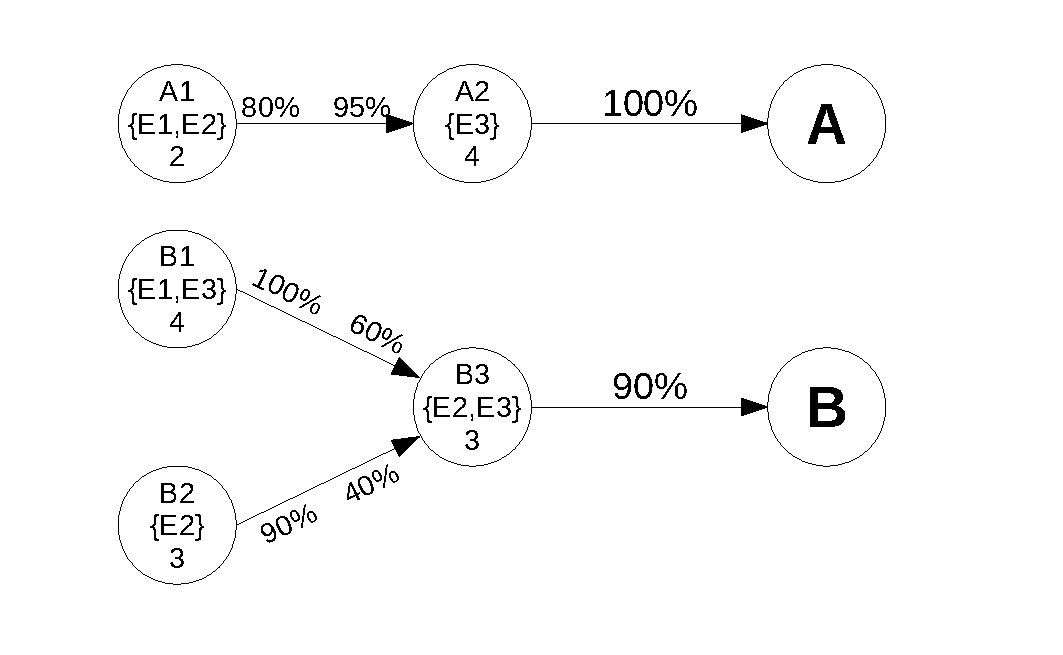
\includegraphics[scale=0.8]{tesztFeladat}
\caption{Tesztfeladat}
\label{tesztFeladat}
\end{center}
\end{figure}

\section{A tesztfeladat megoldása}
A módszer sajátossága, hogy a receptélekkel az egyes taszkok kapacitásának meghatározott százaléka hasznosítható. Ezeket a százalékokat a bemeneti fájlban kell megadni. A példafeladat a~\ref{bemenet1} ábrán megtekinthető bemeneti adatokkal rendelkezik. Az időhorizont a bemutatott mintafeladat során 15. Látható, hogy az egyes részfeladat által lehetséges kapacitásoknak nem a teljes mennyisége kerül tovább a következő taszkhoz. Az, hogy kisebb mennyiség kerül felhasználásra nagy mértékben befolyásolja a korlátot. Emellett az ütemezés megoldását is befolyásolja, mert emiatt lehetséges, hogy bizonyos berendezések nem végezhetik el az adott taszkot.

Az egyszerűség kedvéért a példában csak 2 darab termék receptje szerepel. Az A termék legyártásából származó jövedelem egy egység, a B termék esetén pedig 2 egység. A \textit{precendce} táblában látható, hogy a taszkok által elérhető mennyiségek nem 100 százalékban kerülnek további felhasználásra. Például az A1 és A2 taszkok esetében, az A1-es taszk mennyiségének 80 százaléka kerül továbbításra, illetve ennek a már kisebb mennyiségnek a 95 százalékát veszi fel az A2-es részfeladat. A \textit{proctime} táblán megtalálhatjuk, hogy melyik taszkot, melyik berendezés tudja elvégezni, valamint ezt mennyi idő alatt teszi.
 
\begin{figure}[H]
\begin{center}
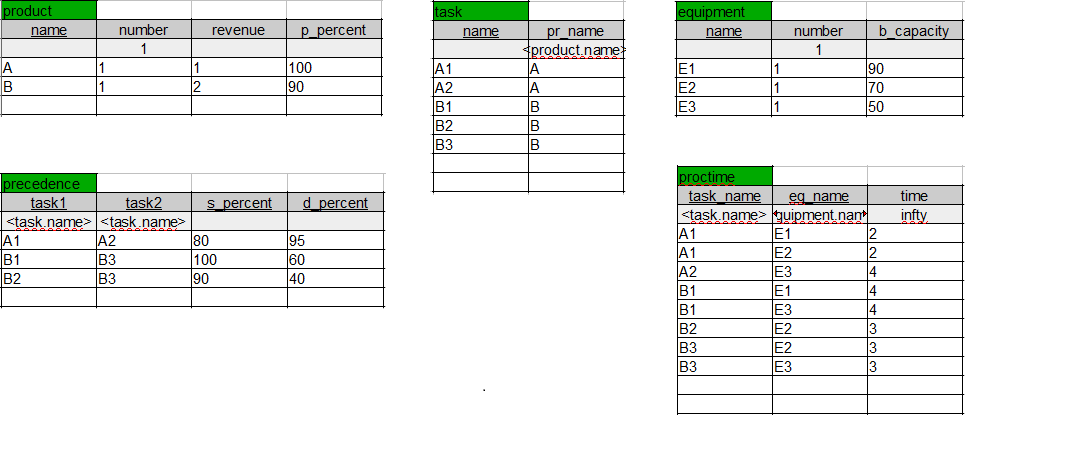
\includegraphics[scale=0.7]{bemenet1}
\caption{A tesztfeladat bemeneti adatai}
\label{bemenet1}
\end{center}
\end{figure}

A feladat megoldását tartalmazó TXT kiterjesztésű fájlt három darab elkülöníthető részre tudjuk felosztani. Az első része látható a~\ref{eredmeny1} ábrán. Az ábra elején az éleket találhatjuk meg, mégpedig olyan formában, hogy melyik taszkból melyik taszkba mutat. Továbbá láthatóak időértékek, amelyek megadják, hogy az élt megelőző részfeladatot mennyi idő alatt lehet elvégezni. Ez a rész tartalmazza mind a receptéleket, mind az ütemezési éleket. Úgy tudjuk ezeket elkülöníteni, hogy amelyikhez 0 időérték van rendelve, azok tartoznak az ütemezési élek csoportjához. Mivel az egyik termékből, nevezetesen az B-ből, több mint egy darabot gyártunk ezért megkülönböztetjük az egyes receptekhez tartozó feladatokat. Láthatunk B1-et és B1\textunderscore 2-t. Ugyanolyan típusú feladatról beszélünk, de különböző recepthez tartoznak, ezért kell megkülönböztetni egymástól ezeket.
 
\begin{figure}[H]
\begin{center}
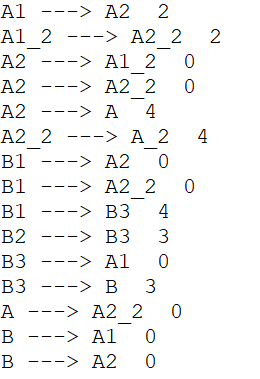
\includegraphics[scale=1]{eredmeny1}
\caption{A megoldást tartalmazó fájl első része}
\label{eredmeny1}
\end{center}
\end{figure}

A második részben a taszkok és a hozzájuk tartozó kapacitások, valamint a termékekhez tartozó kapacitások és a termékek előállításából származó jövedelem szorzata található. Ezeket követően szerepel a bound, a korlát, ami az adott feltételek és adatok mellett 482 lett. Ezt úgy kapjuk meg, hogy a termékekhez tartozó értékeket összeadjuk. Jelen példa esetében 3 érték kerül összeadásra, ezek a következők: A, B és B\textunderscore 2. Az A termékből származó jövedelem 50, a B és a B\textunderscore 2 termékek esetén 216. Ezeket összeadva kijön a 482. Ezek az értékek a~\ref{eredmeny2} ábrán megtekinthetőek.

\begin{figure}[H]
\begin{center}
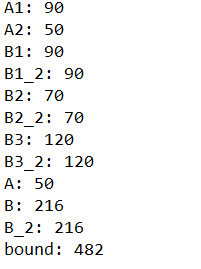
\includegraphics[scale=1.1]{eredmeny2}
\caption{A megoldást tartalmazó fájl második része}
\label{eredmeny2}
\end{center}
\end{figure}

Az utolsó szakaszban a Gantt diagram karakteres formában található meg. Látható, hogy vannak olyan taszkok, amelyeket több berendezés is el tud végezni. A \ref{eredmeny3} ábrán látható ez.

\begin{figure}[H]
\begin{center}
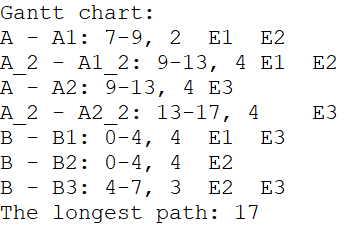
\includegraphics[scale=1]{eredmeny3}
\caption{A megoldást tartalmazó fájl harmadik része}
\label{eredmeny3}
\end{center}
\end{figure}

A \ref{kimenet} ábrán pedig a PNG kiterjesztésű fájl látható. Azonos színnel jelölt taszkok tartoznak egy termékhez. Ha az egyik termékből több példány készül, akkor a termékhez tartozó taszkok végéhez illesztett szám mutatja meg, hogy melyik termékhez tartoznak ezek. A diagramon könnyen észrevehető az új módszerben lévő újítás. A zölddel jelzett B3\_2-es taszk, valamint a kék színű B3-as taszk két berendezéshez, nevezetesen az E2 és az E3 berendezéshez is hozzá lett rendelve. 
\begin{figure}[H]
\begin{center}
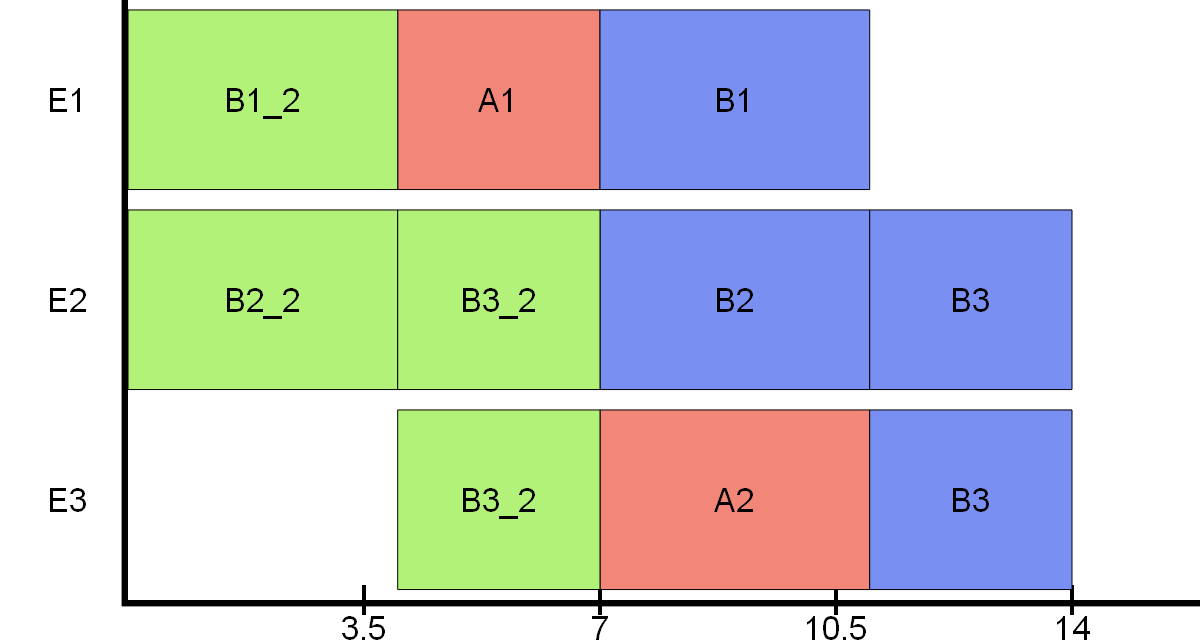
\includegraphics[scale=0.5]{kimenet}
\caption{A solver által elkészített Gantt diagram}
\label{kimenet}
\end{center}
\end{figure}

\section{A régi és az új megoldó összehasonlítása}
Ebben az alfejezetben az eddig meglévő throughput maximalizáló megoldót hasonlítom össze az általam létrehozottal. Ehhez \ref{tesztFeladat} ábrán látható feladatot veszem igénybe. Mivel ebben a feladatban a termékek változó batch mérettel rendelkeznek, ezért a régi megoldó módszerhez szükség van a 3. fejezetben bemutatott diszkretizálás végrehajtására. Ezt elvégezve eredményül azt kapjuk, hogy az A termék gyártása esetén mindenképpen 50 jövedelemre tudunk szert tenni. B termékhez viszont 4 különböző recept jött létre, amelyek mind eltérő jövedelmet biztosítanak. Ezek alapján felrajzolható a 4 gráf, amelyek a \ref{regi_grafok} ábrán láthatóak.
\begin{figure}[H]
\begin{center}
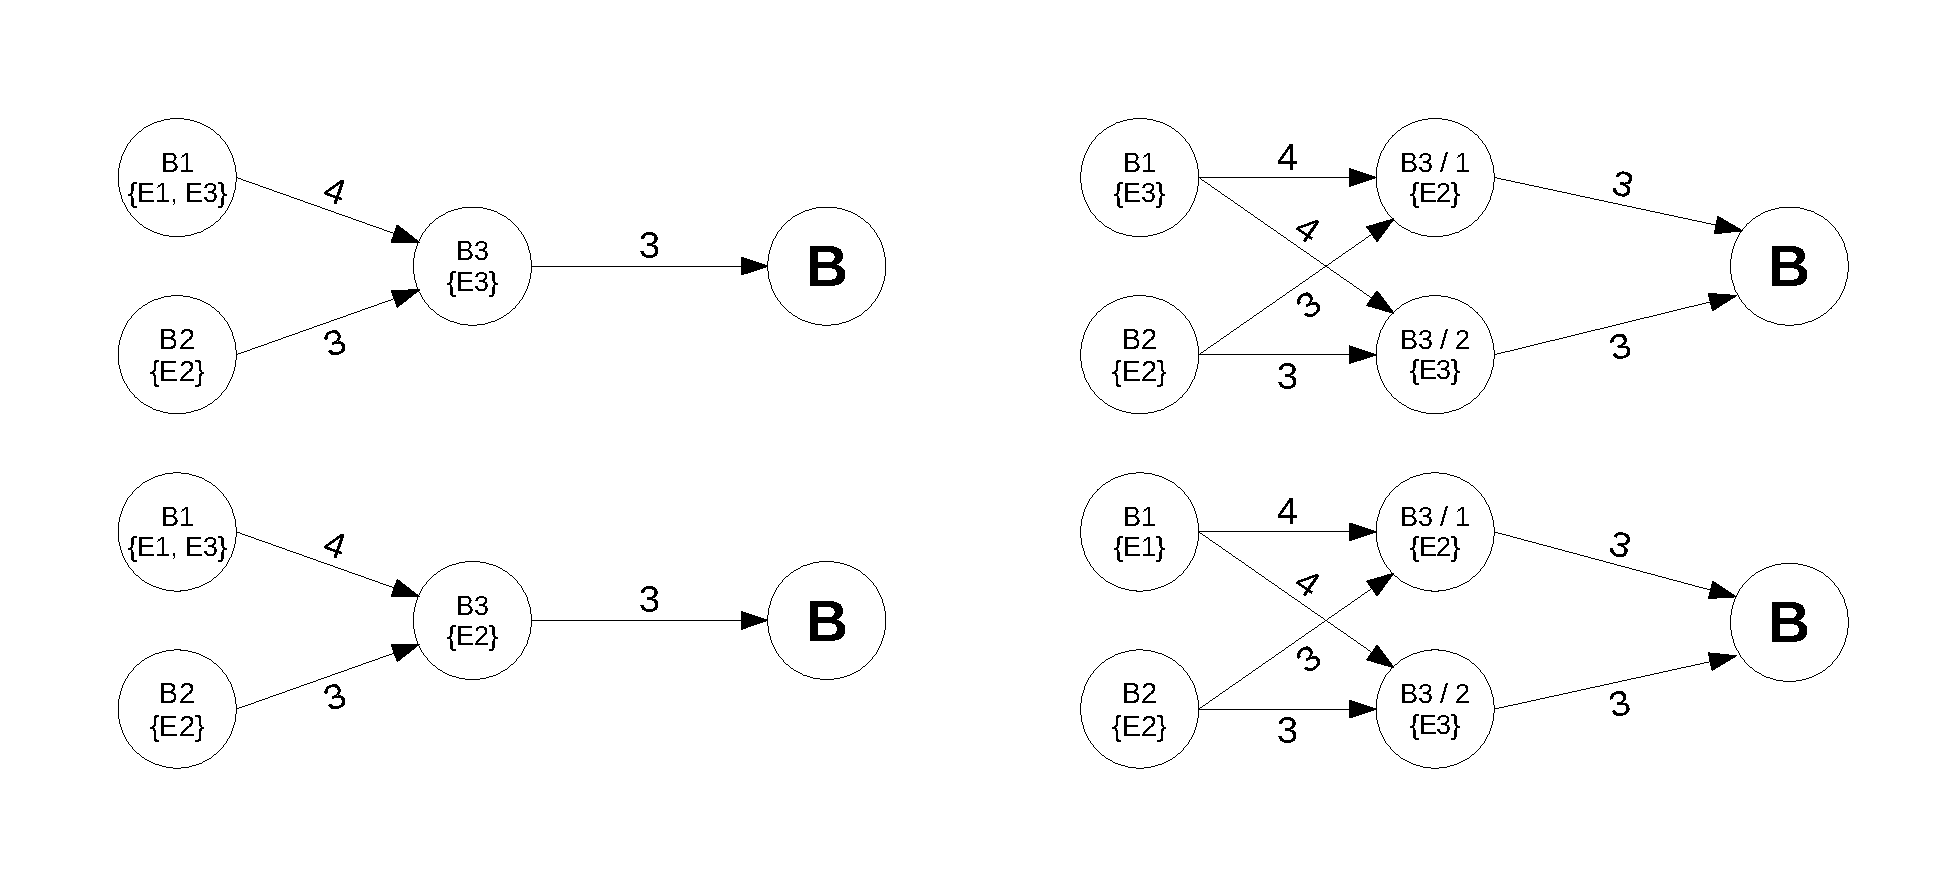
\includegraphics[scale=0.5]{regi_grafok}
\caption{Régi módszer esetén a B termékhez tartozó 4 gráf}
\label{regi_grafok}
\end{center}
\end{figure}
Az ábra bal oldalán szereplő gráfok megegyeznek a példafeladaton szereplő gráffal. Eltérés csak a taszkokat elvégezni tudó berendezésekben van. Azokat a  taszkokat, amelyeket 2 darab berendezés is el tud végezni, úgy kell figyelembe venni, hogy vagy az egyik vagy a másik berendezés végezi majd el az ütemezés után. A jobb oldalon látható, hogy a B3-as taszkból kettő darab lesz. Ezek az estek az jelentik, hogy mindkét berendezés elvégzi ezt a részfeladatot. A régi módszer esetén úgy tekintünk a termékekre, mintha 5 különböző termék lenne. Ezt az 1 darab A termék receptje és a 4 darab különböző B termék receptje adja meg. Ezek alapján elkészíthető a régi megoldóhoz szükséges bemeneti fájl, amely a következő ábrán látható. 

\begin{figure}[H]
\begin{center}
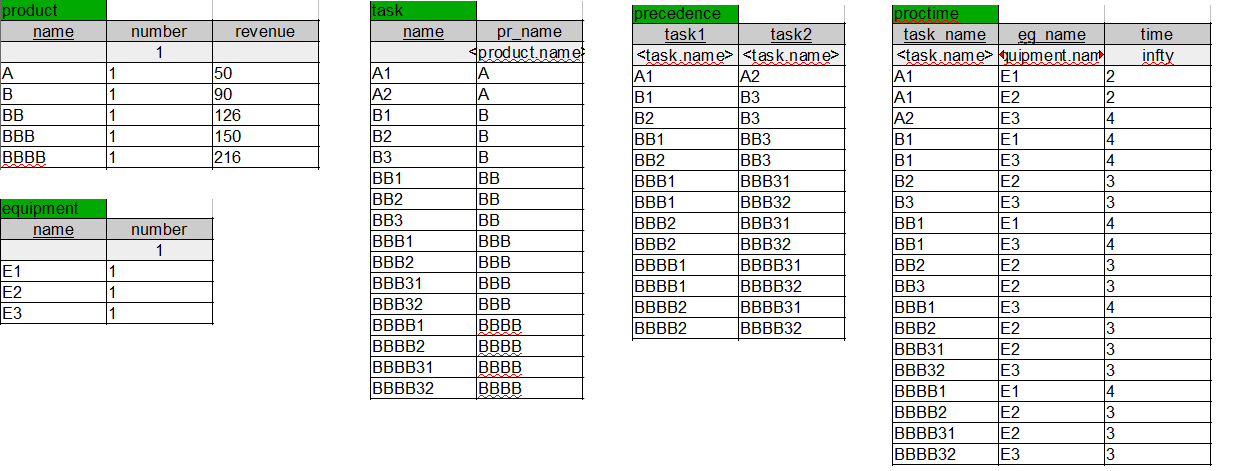
\includegraphics[scale=0.6]{regi_bemenet}
\caption{A régi megoldó bemeneti adatai}
\label{regi_bemenet}
\end{center}
\end{figure}

Látható, hogy ilyen típusú feladat esetében jóval több adat van a fájlban. Ennek az oka a több recept, ami több taszkot és élt jelent. Itt az 5 darab termék miatt egy 5 dimenziós teret lehet elképzelni. Az új megoldó módszernél ez csak 2 dimenziós tér lesz. Láthatjuk, hogy kevesebb dimenziót kell megvizsgálni, viszont egy dimenzión belül több számítást végez el az algoritmus a különböző hozzárendelési lehetőségek miatt. 

Az algoritmus lefutásának végeztével azt várjuk, hogy a régi és az új megoldó ugyanazt az eredményt szolgáltassa. Pontosítva a jövedelem mennyisége és a legyártott termékeknek meg kell egyezniük, a taszkok ütemezésétől azonban ezt nem várjuk el. A \ref{regi_kimenet} ábrán látható a régi megoldómódszer által elkészített Gantt diagram. Összehasonlítva a \ref{kimenet} ábrán látható diagrammal meg lehet állapítani azt, hogy mindkét esetben 2 B termék és 1 darab A terméket lehet legyártani a megadott időhorizonton belül. A másik fontos dolog, hogy a jövedelem is megegyezzen. Az új megoldónál ez 482 volt. A régi által nyújtott eredményben az A termék jövedelme 50, a két B termékből pedig olyanokat gyárt, amelyeknek 216 a jövedelme. Ezeket összeadva, 2 * 216 + 50, itt is kijön a 482. Az ütemezés során a taszkok sorrendje a két megoldó módszer esetén eltér, azonban ez nem hiba. Lehetnek olyan feladatok, ahol ez is teljes mértékben megegyezik.
\begin{figure}[H]
\begin{center}
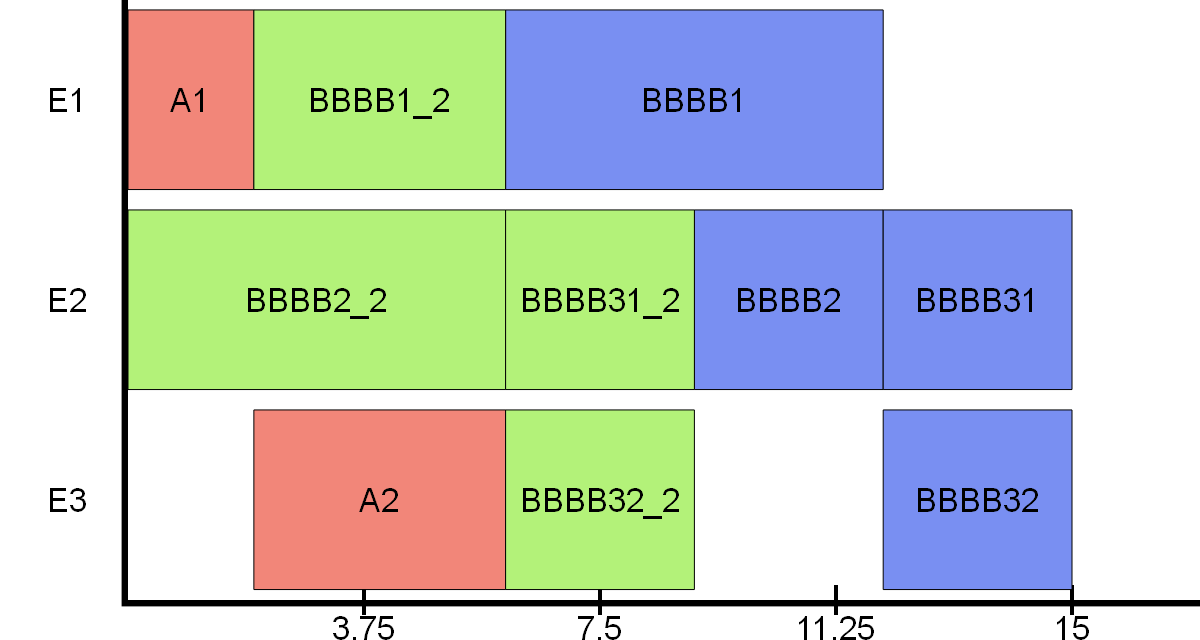
\includegraphics[scale=0.6]{regi_kimenet}
\caption{A régi megoldó által nyújtott Gantt diagram}
\label{regi_kimenet}
\end{center}
\end{figure}

\section{A megoldó módszerek sebessége}
A következő táblázatban a megoldó módszerek sebességének összehasonlítása látható. A régi módszerbe már több, különböző gyorsítási megoldás be van építve. Ezek közé tartozik a korábban már említett precycle és presolver. Az új módszer esetén ezek a gyorsítások jelen állapotban nem működnek. Egy másik kiemelt fontosságú gyorsítás a régi megoldó módszer esetében a revenue line. Ez alsó korlátként szolgál az egyes konfigurációkból származó jövedelmek összehasonlításához. Ennek segítségével, feladattól függően, nagy számú konfiguráció eltávolítható a keresési térből, így jelentősen csökkenthető a számítások mennyisége az ütemezés során. Az új módszer használata során azonban ezt nem vehetjük igénybe, mert nem egy egyenesen szerepelnek azok a konfigurációk, amelyek azonos jövedelemmel rendelkeznek. 

\begin{table}[H]
	\begin{center}
	\caption{Különböző módszerekkel megoldott feladatok összehasonlítása}
	\captionsetup[table]{skip=10pt}
	\label{teszteredmenyek}
\begin{tabular}{|l|l|c|c|c|c|}
\hline
                                                 & \multicolumn{1}{c|}{Megoldó módszer} & Futás ideje          & Time Horizon & Legyártott termék & Profit \\ \hline
\multicolumn{1}{|c|}{\multirow{9}{*}{\rotatebox{90}{Feladat 1}}} & Új                                   & 1,057 mp             & 15           & 1A+2B             & 482    \\ \cline{2-6} 
\multicolumn{1}{|c|}{}                           & Régi                                 & 0,149 mp             & 15           & 1A+2B             & 482    \\ \cline{2-6} 
\multicolumn{1}{|c|}{}                           & Régi (gy. n.)                        & 0,185 mp             & 15           & 1A+2B             & 482    \\ \cline{2-6} 
\multicolumn{1}{|c|}{}                           & Új                                   & 94,964 mp            & 20           & 1A+3B             & 698    \\ \cline{2-6} 
\multicolumn{1}{|c|}{}                           & Régi                                 & 8,17 mp              & 20           & 1A+3B             & 698    \\ \cline{2-6} 
\multicolumn{1}{|c|}{}                           & Régi (gy. n.)                        & 13,553 mp            & 20           & 1A+3B             & 698    \\ \cline{2-6} 
\multicolumn{1}{|c|}{}                           & Új                                   & \textgreater 8000 mp & 25           & 4B                & 864    \\ \cline{2-6} 
\multicolumn{1}{|c|}{}                           & Régi                                 & 705,439 mp           & 25           & 4B                & 864    \\ \cline{2-6} 
\multicolumn{1}{|c|}{}                           & Régi (gy. n.)                        & 1175,11 mp           & 25           & 4B                & 864    \\ \hline
\multirow{9}{*}{\rotatebox{90}{Feladat 2}}                      & Új                                   & 0,371 mp             & 15           & 2C+1D             & 188    \\ \cline{2-6} 
                                                 & Régi                                 & 0,07 mp              & 15           & 2C+1D             & 188    \\ \cline{2-6} 
                                                 & Régi (gy. n.)                        & 0,113 mp             & 15           & 2C+1D             & 188    \\ \cline{2-6} 
                                                 & Új                                   & 15,486 mp            & 20           & 3C+1D             & 252    \\ \cline{2-6} 
                                                 & Régi                                 & 1,306 mp             & 20           & 3C+1D             & 252    \\ \cline{2-6} 
                                                 & Régi (gy. n.)                        & 3,201 mp             & 20           & 3C+1D             & 252    \\ \cline{2-6} 
                                                 & Új                                   & 741,29 mp            & 25           & 3C+3D             & 360    \\ \cline{2-6} 
                                                 & Régi                                 & 58,28 mp             & 25           & 3C+3D             & 360    \\ \cline{2-6} 
                                                 & Régi (gy. n.)                        & 222,679 mp           & 25           & 3C+3D             & 360    \\ \hline
\multirow{6}{*}{\rotatebox{90}{Feladat 3}}                       & Új                                   & 14,78 mp             & 10           & 2H+2I             & 86     \\ \cline{2-6} 
                                                 & Régi                                 & 0,374 mp             & 10           & 2H+2I             & 86     \\ \cline{2-6} 
                                                 & Régi (gy. n.)                        & 0,381 mp             & 10           & 2H+2I             & 86     \\ \cline{2-6} 
                                                 & Új                                   & 44,693 mp            & 15           & 4I                & 94     \\ \cline{2-6} 
                                                 & Régi                                 & 0,985 mp             & 15           & 4I                & 94     \\ \cline{2-6} 
                                                 & Régi (gy. n.)                        & 0,806 mp             & 15           & 4I                & 94     \\ \hline
\end{tabular}
\end{center}
\end{table}

Ugyanaz a feladat 3 módszerrel került megoldásra. A régivel, amelyben szerepelnek a gyorsítások, ismét a régi megoldóval (régi gy. n.), de itt a precycle és a presolver gyorsítások nélkül, illetve az elkészített új megoldó módszerrel. Látható, hogy a régi módszerek gyorsabban találjak meg a feladat legjobb megoldását, mint az új a jelenlegi állapotában. Jövőbeni tervek közé tartozik a meglévő gyorsítások átalakítása, hogy kompatibilisek legyenek az új módszerrel is. Ezek megvalósítása után nagy csökkenés várható az új megoldó módszer futási idejében. 